

In questo capitolo vengono introdotti i bilanci di alcune quantità meccaniche per un mezzo continuo. I bilanci in forma integrale permettono di descrivere l'evoluzione complessiva (integrale) di un sistema e vengono ricavati partendo da alcuni principi fondamentali della meccanica classica: la conservazione della massa, l'equazioni cardinali della dinamica, il primo principio della termodinamica o bilancio dell'energia. Vengono scritti prima per un volume materiale e poi per volumi di controllo o volumi in moto generico, utilizzando il teorema del trasporto di Reynolds.

\noindent
Dai bilanci in forma integrale, sotto ipotesi di sufficiente regolarità dei campi, vengono poi ricavati i bilanci in forma differenziale, che permettono di descrivere l'evoluzione locale (puntuale) di un sistema. La forma lagrangiana del bilanci di massa, di quantità di moto e della vorticità verrà utilizzata per meglio apprezzare il significato del vincolo di incomprimibilità, il ruolo della pressione (e degli sforzi in generale) nella dinamica di un fluido e intuire l'influenza del campo di velocità sul campo di vorticità.

\noindent
Successivamente, dai bilanci integrali vengono ricavate le relazioni di salto delle quantità meccaniche. Queste relazioni possono essere utilizzate per trovare determinare lo stato di un sistema formato da due sotto-sistemi, all'interno dei quali i campi sono regolari, ma che sono separati da una frontiera, attraverso la quale i campi non sono regolari: alcuni esempi di queste sono le superfici ``di scorrimento'' in fluidi non viscosi, attraverso le quali è discontinua la componente tangenziale della velocità, o le onde d'urto che possono formarsi in correnti comprimibili di fluidi non viscosi.

\noindent
Infine, viene fornita una breve introduzione agli esercizi sui bilanci integrali, che costituisce una prima linea guida al loro svolgimento.

%In fondo alla sezione viene data una lettura ``non convenzionale'' di alcuni bilanci e vengono ricavate le relazioni di salto delle grandezze meccaniche attraverso superfici di discontinuità, dove le equazioni in forma differenziale non sono valide. La scrittura in forma lagrangiana dei bilanci di massa, di quantità di moto e di vorticità permette di apprezzare il concetto di incomprimibilità, intuire il ruolo della pressione (e dello sforzo) nel determinare la traiettoria di una particella fluida e intuire il legame tra evoluzione della vorticità e del campo di velocità.
% Le relazioni di salto verranno usate nel capitolo successivo per ricavare le grandezze attraverso superfici di discontinuità \textit{di contatto}, ma risultano valide anche attraverso le discontinuità (onde d'urto) che si formano nel campo di moto quando gli effetti viscosi sono trascurabili.


\section{Bilanci in forma integrale}

Vengono ricavati i bilanci integrali per un volume materiale $V(t)$ partendo dai principi fondamentali della meccanica classica. Successivamente si ricavano i bilanci per un volumi in moto arbitrario $v(t)$ e, come caso particolare, volumi di controllo $V_c$.

\subsection{Bilancio di massa}
La massa di un volume materiale è uguale all'integrale sul volume della densità $\rho$. Per il \textbf{principio di conservazione della massa}, la massa di un sistema chiuso (che non ha scambi di materia con l'esterno), come ad esempio un volume materiale $V(t)$, rimane costante e quindi la sua derivata nel tempo deve essere uguale a zero,
\begin{fBox}
\begin{equation}
 \dfrac{d}{dt} \int_{V(t)} \rho = 0 \ .
\end{equation}
\end{fBox}

\subsection{Bilancio della quantità di moto}
La quantità di moto di un volume materiale è uguale all'integrale sul volume della quantità di moto per unità di volume $\rho \bm{u}$, dove $\bm{u}$ è la velocità delle particelle materiali.
Per la \textbf{prima equazione cardinale della dinamica}, la derivata nel tempo della quantità di moto di un sistema è uguale alla risultante delle forze esterne agenti sul sistema,
\begin{fBox}
\begin{equation}
 \dfrac{d}{dt} \int_{V(t)} \rho \bm{u} = \int_{V(t)} \bm{f} + \oint_{S(t)} \bm{t_n} \ , 
\end{equation}
\end{fBox}
dove $\int_{V(t)} \bm{f}$ rappresenta la risultante delle forze esterne di volume e $\oint_{S(t)} \bm{t_n}$ la risultante delle forze esterne di superficie, avendo indicato con $\bm{f}$ il campo di forze per unità di volume e $\bm{t_n}$ il vettore sforzo agente sulla supreficie esterna $S(t)$ del volume $V(t)$. Il teorema di Cauchy nella meccanica del continuo, permette di esprimere il vettore sforzo $\bm{t_n}$ in funzione del tensore degli sforzi $\mathbb{T}$ e la normale alla superficie $\bm{\hat{n}}$, come $\bm{t_n} = \bm{\hat{n}} \cdot \mathbb{T}$.

\subsection{Bilancio del momento quantità di moto}

Il momento della quantità di moto di un volume materiale è uguale all'integrale sul volume del momento della quantità di moto per unità di volume $\rho \bm{r} \times \bm{u}$, dove $\bm{r}$ è il vettore che congiunge il polo con i punti del volume materiale.
Per la \textbf{seconda equazione cardinale della dinamica}, la derivata nel tempo del momento della quantità di moto di un sistema, rispetto a un polo fisso, è uguale alla risultante momenti esterni sul sistema,
\begin{fBox}
\begin{equation}
 \dfrac{d}{dt} \int_{V(t)} \rho \bm{r} \times \bm{u} = \int_{V(t)} \bm{r} \times \bm{f} + \oint_{S(t)} \bm{r} \times \bm{t_n} \ , 
\end{equation}
\end{fBox}
nell'ipotesi che non ci siano momenti esterni per unità di volume e che il materiale non sia polare (due elementi di materiale adiacenti non si scambiano momenti ma solo forze).

\subsection{Bilancio dell'energia totale}

L'energia totale di un volume materiale è uguale all'integrale sul volume della sua energia interna per unità di volume $\rho e$ e della sua energia cinetica per unità di volume $\rho |\bm{u}|^2/2$. Combinando il \textbf{primo principio della termodinamica} (che riguarda solo sistemi in equilibrio) con il \textbf{teorema dell'energia cinetica} (che non include il contributo di energia interna), la derivata nel tempo dell'energia totale del sistema di un sistema è uguale alla differenza tra la potenza delle forze agenti sul sistema e i flussi di calore uscenti da esso,
\begin{fBox}
\begin{equation}
 \dfrac{d}{dt} \int_{V(t)} \rho e^t = \int_{V(t)} \bm{f} \cdot \bm{u} + \oint_{S(t)} \bm{t_n} \cdot \bm{u} - \oint_{S(t)} \bm{q} \cdot \bm{\hat{n}} + \int_{V(t)} \rho r \ , 
\end{equation}
\end{fBox}
avendo indicato con $\bm{q}$ il flusso di calore uscente dal volume materiale $V(t)$, e con $r$ l'intensità di una sorgente di calore per unità di massa $r$, distributia all'interno del volume $V(t)$, come ad esempio il calore rilasciato da una reazione chimica come la combustione.

\subsection{Bilanci integrali per volumi in moto arbitrario}
Utilizzando il teorema del trasporto di Reynolds, è possibile esprimere la derivata nel tempo dell'integrale di un campo $f$ su un volume materiale $V(t)$ come somma della derivata nel tempo dell'integrale dello stesso campo $f$ su un volume arbitrario $v(t)$ e al flusso della quantità $f$ attraverso la frontiera $s(t)=\partial v(t)$ di $v(t)$, dovuto alla velocità relativa $\bm{u} - \bm{v}$ tra le particelle materiali e la superficie $s(t)$,
%\begin{fBox}
\begin{equation}
  \dfrac{d}{d t} \int_{V(t)} f = \dfrac{d}{d t} \int_{v(t)\equiv V(t)} f +
 \oint_{s(t)\equiv S(t)} f (\bm{u} - \bm{v}) \cdot \bm{\hat{n}} \ .
\end{equation}
%\end{fBox}

\noindent
I bilanci integrali riferiti a un volume arbitrario $v(t)$, la cui superficie $s(t)$ si muove con velocità $\bm{v}$, risultano
\begin{equation}
\begin{cases}
 \dfrac{d}{dt} \displaystyle\int_{v(t)} \rho + \oint_{s(t)} \rho (\bm{u}-\bm{v}) \cdot \bm{\hat{n}}= 0  \\
 \dfrac{d}{dt} \displaystyle\int_{v(t)} \rho \bm{u} + \oint_{s(t)} \rho \bm{u} (\bm{u} - \bm{v}) \cdot \bm{\hat{n}} = \int_{v(t)} \bm{f} + \oint_{s(t)} \bm{t_n}  \\
 \dfrac{d}{dt} \displaystyle\int_{v(t)} \rho \bm{r} \times \bm{u} + \oint_{s(t)} \rho \bm{r} \times \bm{u} (\bm{u}-\bm{v}) \cdot \bm{\hat{n}}= \int_{v(t)} \bm{r} \times \bm{f} + \oint_{s(t)} \bm{r} \times \bm{t_n} \\
 \dfrac{d}{dt} \displaystyle\int_{v(t)} \rho e^t + \oint_{s(t)} \rho e^t (\bm{u}-\bm{v}) \cdot \bm{\hat{n}}= \int_{v(t)} \bm{f} \cdot \bm{u} + \oint_{s(t)} \bm{t_n} \cdot \bm{u} - \oint_{s(t)} \bm{q} \cdot \bm{\hat{n}} + \int_{V(t)} \rho r \ .
\end{cases}
\end{equation}

\subsection{Bilanci integrali per volumi di controllo fissi}

Come caso particolare dei bilanci integrali riferiti a un volume arbitrario $v(t)$,  i bilanci integrali riferiti a un volume di controllo fisso $V_c$ risultano
\begin{equation}
 \begin{cases}
   \dfrac{d}{d t} \displaystyle\int_{V_c} \rho + \oint_{S_c} \rho \bm{u} \cdot \bm{\hat{n}} = 0 \\
   \dfrac{d}{d t} \displaystyle\int_{V_c} \rho  \bm{u}+ \oint_{S_c} \rho \bm{u} \bm{u} \cdot \bm{\hat{n}} = \int_{V_c} \bm{f} + \oint_{S_c} \bm{t_n} \\
   \dfrac{d}{d t} \displaystyle\int_{V_c} \rho \bm{r} \times \bm{u}+ \oint_{S_c} \rho \bm{r} \times \bm{u} \bm{u} \cdot \bm{\hat{n}} = \int_{V_c} \bm{r} \times \bm{f} + \oint_{S_c} \bm{r} \times \bm{t_n} \\
   \dfrac{d}{d t} \displaystyle\int_{V_c} \rho e^t + \oint_{S_c} \rho e^t \bm{u} \cdot \bm{\hat{n}} = \int_{V_c} \bm{f} \cdot \bm{u} + \oint_{S_c} \bm{t_n} \cdot \bm{u} - \oint_{S_c} \bm{q} \cdot \bm{\hat{n}} + \int_{V(t)} \rho r  \ .
 \end{cases}
\end{equation}


\section{Bilanci in forma differenziale}

Sotto le ipotesi di sufficiente regolarità dei campi che compaiono negli integrali di superficie, è possibile trasformare gli integrali di superficie in integrali di volume, applicando il teorema della divergenza o il lemma del teorema di Green
\begin{equation}
  \oint_{S} f n_i = \int_V f_{/i} \ ,
\end{equation}
 avendo indicato con $f_{/i}$ la derivata parziale rispetto alla coordinata cartesiana $x_i$ e con $n_i$ la proiezione lungo $x_i$ della normale uscente dalla superficie $S=\partial V$.
Una volta scritti tutti i termini come integrali di volume, sullo stesso volume $V$, è possibile sfruttare l'arbitrarietà del volume $V$ per ricavare i bilanci in forma differenziale.
In questa sezione, si partirà dai bilanci in forma integrale scritti per un volume di controllo fisso $V=V_c$, per il quale vale
\begin{equation}
 \dfrac{d}{d t} \int_V f = \int_V \dfrac{\partial f}{\partial t} \ ,
\end{equation}
secondo il teorema del trasporto di Reynolds.

\subsection{Bilancio di massa}
Usando il teorema del trasporto di Reynolds per volumi di controllo fissi e applicando il teorema della divergenza al termine di flusso, si può scrivere
\begin{equation}
 \dfrac{d}{d t} \displaystyle\int_{V} \rho + \oint_{S} \rho \bm{u} \cdot \bm{\hat{n}} = \int_V \left[ \dfrac{\partial \rho}{\partial t} + \bm{\nabla} \cdot (\rho \bm{u})\right] = 0 \ .
\end{equation}
Sfruttando l'arbitrarietà del bilancio integrale dal volume considerato e imponendo che l'integranda sia nulla, si ricava la \textit{forma conservativa} del bilancio differenziale di massa,
\begin{fBox}
\begin{equation}
  \dfrac{\partial \rho}{\partial t} + \bm{\nabla} \cdot (\rho \bm{u}) = 0 
\end{equation}
\end{fBox}
Sviluppando la divergenza $\bm{\nabla} \cdot (\rho \bm{u}) = \rho \bm{\nabla} \cdot \bm{u} + \bm{u} \cdot \bm{\nabla} \rho$, e riconoscendo l'espressione della derivata materiale, si ottiene la \textit{forma convettiva} del bilancio differenziale di massa,
\begin{fBox}
\begin{equation}
\begin{aligned}
 \dfrac{\partial \rho}{\partial t} + \bm{u} \cdot \bm{\nabla} \rho &+ \rho \bm{\nabla} \cdot \bm{u} = 0 \\ 
 \dfrac{D \rho}{D t} = &- \rho \bm{\nabla} \cdot \bm{u} \ .
\end{aligned}
\end{equation}
\end{fBox}
Il vincolo cinematico di incomprimibilità $\bm{\nabla} \cdot \bm{u} = 0$ equivale al vincolo ``fisico'' che impone che la densità delle singole particelle materiali rimanga costante, $D\rho/Dt = 0$.

\subsection{Bilancio di quantità di moto}
\'E possibile trasformare in un integrale di volume la risultante degli sforzi di superficie, utilizzando il teorema di Cauchy per i mezzi continui, 
\begin{equation}
  \bm{t_n} = \bm{\hat{n}} \cdot \mathbb{T} \quad , \quad 
  t_i = n_j T_{ji} \ ,
\end{equation}
dove $\bm{t_n}$ è il vettore sforzo, $\bm{\hat{n}}$ la normale alla superficie e $\mathbb{T}$ il tensore degli sforzi.
La risultante degli sforzi di superficie diventa, usando un po' di libertà nel passare dalla notazione astratta a quella indiciale,
\begin{equation}
 \oint_S \bm{t_n} = \oint_S t_i = \oint_S n_j T_{ji} =
  \int_V T_{ji/j} = \int_V \bm{\nabla} \cdot \mathbb{T} \ .
\end{equation}
Usando il teorema del trasporto di Reynolds per volumi di controllo fissi e applicando il teorema della divergenza al termine di flusso,
\begin{equation}
 \oint_S \big\{ \rho \bm{u} \bm{u} \cdot \bm{\hat{n}} \big\}_i = \oint_S \rho u_i u_j n_j = \int_V (\rho u_i u_j)_{/j} = \int_{V} \bm{\nabla} \cdot ( \rho \bm{u} \otimes \bm{u} ) \ ,
\end{equation}
si può scrivere il bilancio di quantità di moto 
\begin{equation}
  \displaystyle\int_{V} \dfrac{\partial(\rho \bm{u})}{\partial t}  + \int_{V} \bm{\nabla} \cdot ( \rho \bm{u} \otimes \bm{u} ) = \int_{V} \left[ \bm{f} +  \bm{\nabla} \cdot \mathbb{T} \right] \ .
\end{equation}
Sfruttando l'arbitrarietà del bilancio integrale dal volume considerato e imponendo che l'integranda sia nulla, si ricava la \textit{forma conservativa} del bilancio differenziale di quantità di moto,
\begin{fBox}
\begin{equation}
 \dfrac{\partial(\rho \bm{u})}{\partial t}  + \bm{\nabla} \cdot ( \rho \bm{u} \otimes \bm{u} - \mathbb{T} ) = \bm{f} \ .
\end{equation}
\end{fBox}
Sviluppando i termini 
\begin{equation}
\begin{aligned}
 \dfrac{\partial (\rho \bm{u})}{\partial t} = \rho \dfrac{\partial \bm{u}}{\partial t} + \bm{u} \dfrac{\partial \rho}{\partial t} \quad & , \quad 
 \dfrac{\partial (\rho u_i)}{\partial t} = \rho \dfrac{\partial u_i}{\partial t} + u_i \dfrac{\partial \rho}{\partial t} \\
 \bm{\nabla} \cdot ( \rho \bm{u} \otimes \bm{u} ) = \rho (\bm{u} \cdot \bm{\nabla}) \bm{u} + \bm{u} \bm{\nabla} \cdot (\rho \bm{u}) \quad & , \quad 
 ( \rho u_i u_j )_{/j} = \rho u_j u_{i/j} + u_i (\rho u_j)_{/j} 
  \ ,
\end{aligned}
\end{equation} 
 riconoscendo che $\bm{u} \cdot (\partial \rho/\partial t + \bm{\nabla} \cdot (\rho \bm{u}))=0$ come conseguenza della conservazione della massa, si ottiene la \textit{forma convettiva} dell'equazione della quantità di moto
\begin{fBox}
 \begin{equation}
  \begin{aligned}
   \rho \dfrac{\partial\bm{u}}{\partial t}  +  \rho (\bm{u}  \cdot \bm{\nabla} ) \bm{u}& = \bm{f} + \bm{\nabla} \cdot \mathbb{T}  \\ 
   \rho \dfrac{D \bm{u}}{D t} & = \bm{f} + \bm{\nabla} \cdot \mathbb{T} \ . \\ 
  \end{aligned}
 \end{equation}
\end{fBox}

\subsection{Bilancio del momento della quantità di moto}
Il bilancio del momento della quantità di moto per un mezzo continuo non polare è equivalente alla condizione di simmetria del tensore degli sforzi
\begin{equation}
 \mathbb{T}^T = \mathbb{T} \quad , \quad T_{ij} = T_{ji} \ .
\end{equation}

\subsection{Bilancio dell'energia totale}
Usando un po' di libertà nel passare dalla notazione astratta a quella indiciale, la potenza degli sforzi di superficie diventa
\begin{equation}
\begin{aligned}
 \oint_S \bm{t_n} \cdot \bm{u} = \oint_S t_i u_i = \oint_S n_j T_{ji} u_i & =
  \int_V (T_{ji} u_i)_{/j}= \int_V \bm{\nabla} \cdot ( \mathbb{T} \cdot \bm{u}) \\
  & = \int_V (T_{ij/j} u_i + T_{ij} u_{j/i}) = \int_V \big( (\bm{\nabla} \cdot \mathbb{T}) \cdot \bm{u} + \mathbb{T} : \bm{\nabla} \bm{u} \big) \ , 
\end{aligned} 
\end{equation}
avendo utilizzato la simmetria del tensore degli sforzi, $T_{ij/j} = \{ \bm{\nabla} \cdot \mathbb{T}^T \}_i = \{ \bm{\nabla} \cdot \mathbb{T} \}_i$. Applicando il teorema della divergenza, il termine di flusso di calore viene scritto come
\begin{equation}
 \oint_S \bm{q} \cdot \bm{\hat{n}} = \int_V \bm{\nabla} \cdot \bm{q} \ .
\end{equation}
La \textit{forma conservativa} del bilancio differenziale di energia totale diventa quindi
\begin{fBox}
\begin{equation}
 \dfrac{\partial (\rho e^t)}{\partial t} + \bm{\nabla} \cdot (\rho e^t \bm{u} - \mathbb{T} \cdot \bm{u} + \bm{q}) = \bm{f} \cdot \bm{u} + \rho r \ .
\end{equation}
\end{fBox}
Sviluppando la derivata temporale e il termine $\bm{\nabla} \cdot (\rho e^t \bm{u}) = \rho \bm{u} \cdot \bm{\nabla} e^t + e^t \bm{\nabla} \cdot (\rho \bm{u})$, riconoscendo che $e^t (\partial \rho/\partial t + \bm{\nabla} \cdot (\rho \bm{u}))=0$ come conseguenza della conservazione della massa, si ottiene la \textit{forma convettiva} dell'equazione dell'energia totale,
\begin{fBox}
 \begin{equation}
  \begin{aligned}
   \rho \dfrac{\partial e^t}{\partial t}  +  \rho \bm{u}  \cdot  \bm{\nabla} e^t & = \bm{f} \cdot \bm{u} + \bm{\nabla} \cdot ( \mathbb{T} \cdot \bm{u} ) - \bm{\nabla} \cdot \bm{q} + \rho r \\ 
   \rho \dfrac{D e^t}{D t} & =  \bm{f} \cdot \bm{u} + \bm{\nabla} \cdot ( \mathbb{T} \cdot \bm{u} ) - \bm{\nabla} \cdot \bm{q} + \rho r  \ . \\ 
  \end{aligned}
 \end{equation}
\end{fBox}

\subsection{Chiusura del problema}
Affinché il sistema di equazioni differenziali alle derivate parziali formato dai bilanci di massa, quantità di moto ed energia totale, con le condizioni iniziali e al contorno adeguate, sono necessarie l'equazione di stato del materiale che ne descriva le proprietà termodinamiche\footnote{Si ricorda che lo stato termodinamico di un sistema monofase è definito da due variabili termodinamiche indipendenti.} e i legami costitutivi che esprimano il tensore degli sforzi e il flusso di calore come funzioni dello stato dinamico e termodinamico del sistema.
Per un fluido, il tensore degli sforzi viscosi $\mathbb{T}$ può essere scritto come la somma del contributo idrostatico dovuto alla pressione $p$ e il tensore degli sforzi viscosi $\mathbb{S}$, funzione delle derivate spaziali del campo di velocità. Un fluido che ha un \textit{legame costitutivo lineare} tra il tensore degli sforzi viscosi e il gradiente di velocità $\bm{\nabla} \bm{u}$, viene definito \textbf{fluido newtoniano}. Per un fluido newtoniano isotropo, il legame costitutivo che definisce il tensore degli sforzi è
\begin{equation}
 \mathbb{T} = -p \mathbb{I} + 2 \mu \mathbb{D} + \lambda (\bm{\nabla} \cdot \bm{u}) \mathbb{I} \ ,
\end{equation}
dove $\mu$ e $\lambda$ sono rispettivamente il coefficiente di viscosità dinamica e il secondo coefficiente di viscosità, $p$ è  la pressione (``termodinamica''), $\mathbb{D}$ il tensore velocità di deformazione. In generale, sia la pressione $p$ sia i coefficienti di viscosità dipendono dallo stato termodinamico del sistema. \newline
Il flusso di calore $\bm{q}$ per conduzione può essere descritto dalla \textbf{legge di Fourier}, che lo mette in relazione con il gradiente della temepratura tramite il coefficiente di conduzione termica $k$, in generale funzione dello stato termodinamico del sistema,
\begin{equation}
 \bm{q} = - k \bm{\nabla} T \ .
\end{equation}
L'introduzione di queste leggi costitutive nelle equazioni di bilancio, aggiunge nuove incognite  al sistema, per le quali non abbiamo ricavato un'equazione dinamica. Sono quindi indispensabili la legge di stato che fornisca le relazioni necessarie,
\begin{equation}
 \begin{aligned}
  p = p(\rho,e) \quad , & \quad \mu = \mu(\rho,e) \\
  T = T(\rho,e) \quad , & \quad \lambda = \lambda(\rho,e) \\
  & \quad k = k(\rho,e) \ ,
 \end{aligned}
\end{equation}
avendo scelto le variabili termodinamiche delle quali è nota l'equazione dinamica come due variabili termodinamiche indipendenti: la densità $\rho$ e l'energia interna $e$. Ve


\subsection{Altre equazioni di bilancio}
Combinando i bilanci delle quantità meccaniche ottenuti partendo dai principi fondamentali della fisica, si possono ottenere le equazioni di bilanci di altre quantità, come ad esempio l'energia cinetica $\rho|\bm{u}|^2/2$, l'energia interna $e$, e la vorticità $\bm{\omega} = \nabla \times \bm{u}$.
\paragraph{Equazione dell'energia cinetica} Moltiplicando scalarmente il bilancio della quantità di moto per il vettore velocità $\bm{u}$, si può scrivere l'equazione di bilancio dell'energia cinetica. In forma conservativa,
\begin{fBox}
\begin{equation}
 \dfrac{\partial}{\partial t}\dfrac{\rho|\bm{u}|^2}{2}  + \bm{\nabla} \cdot \left( \rho \bm{u} \dfrac{|\bm{u}|^2}{2} \right) = \bm{f} \cdot \bm{u} + \bm{u} \cdot ( \bm{\nabla} \cdot \mathbb{T} ) \ ,
\end{equation}
\end{fBox}
in forma convettiva,
\begin{fBox}
 \begin{equation}
  \begin{aligned}
   \rho \dfrac{\partial}{\partial t} \dfrac{|\bm{u}|^2}{2} +  \rho \bm{u}  \cdot \bm{\nabla} \dfrac{|\bm{u}|^2}{2} & = \bm{f} \cdot \bm{u} + \bm{u} \cdot (\bm{\nabla} \cdot \mathbb{T} ) \\ 
   \rho \dfrac{D }{D t}\dfrac{|\bm{u}|^2}{2} & = \bm{f}\cdot \bm{u} + \bm{u} \cdot ( \bm{\nabla} \cdot \mathbb{T} ) \ . \\ 
  \end{aligned}
 \end{equation}
\end{fBox}

\paragraph{Equazione dell'energia interna} Dalla differenza del bilancio dell'energia totale e dell'energia cinetica, si ottiene il bilancio dell'energia interna.
In forma conservativa,
\begin{fBox}
\begin{equation}
 \dfrac{\partial (\rho e)}{\partial t} + \bm{\nabla} \cdot (\rho e \bm{u}) = \mathbb{T}:\bm{\nabla}\bm{u} - \bm{\nabla} \cdot \bm{q} + \rho r \ ,
\end{equation}
\end{fBox}
in forma convettiva,
\begin{fBox}
 \begin{equation}
  \begin{aligned}
   \rho \dfrac{\partial e}{\partial t} +  \rho \bm{u}  \cdot \bm{\nabla}e & =  \mathbb{T}:\bm{\nabla}\bm{u} - \bm{\nabla} \cdot \bm{q} + \rho r \\
   \rho \dfrac{D e}{D t} & =  \mathbb{T}:\bm{\nabla}\bm{u} - \bm{\nabla} \cdot \bm{q} + \rho r \ . \\ 
  \end{aligned}
 \end{equation}
\end{fBox}

\paragraph{Equazione della vorticità} Applicando l'operatore di rotore al bilancio della quantità di moto, si ottiene l'equazione dinamica della vorticità. Per un fluido newtoniano (con coefficienti di viscosità costanti e uniformi),
\begin{fBox}
\begin{equation}
\begin{aligned}
 \dfrac{\partial \bm{\omega}}{\partial t} + (\bm{u} \cdot \bm{\nabla} ) \bm{\omega} & =
  (\bm{\omega} \cdot \bm{\nabla}) \bm{u} - \bm{\omega} (\bm{\nabla} \cdot \bm{u}) +
  \nu \Delta \bm{\omega} + \dfrac{\bm{\nabla} \rho \times \bm{\nabla} p}{\rho^2} \\
   \dfrac{D \bm{\omega}}{D t}  & =
  (\bm{\omega} \cdot \bm{\nabla}) \bm{u} - \bm{\omega} (\bm{\nabla} \cdot \bm{u}) +
  \nu \Delta \bm{\omega} + \dfrac{\bm{\nabla} \rho \times \bm{\nabla} p}{\rho^2} \ ,
 \end{aligned}
\end{equation}
\end{fBox}
dove è stata introdotta la viscosità cinematica del fluido, $\nu = \mu / \rho$.

\paragraph{Equazione dell'entropia} Nell'ipotesi di equilibrio termodinamico delle singole particelle materiali\footnote{Se i tempi caratteristici della termodinamica sono di gran lunga inferiori al tempo caratteristico del fenomeno fluidodinamico, si può immaginare che la singola particella fluida sia in continuo stato di equilibrio termodinamico locale. Si possono quindi estendere i risultati della Termodinamica, che in generale studia sistemi in equilibrio, alla singola particella fluida.} si può ricavare dal primo principio della termodinamica,
\begin{equation}
 de = T ds - P dv = T ds + \dfrac{p}{\rho^2} d\rho \ ,
\end{equation}
l'equazione di bilancio dell'entropia in forma convettiva,
\begin{equation}
 T \dfrac{D s}{D t} = \dfrac{D e}{D t} - \dfrac{p}{\rho^2} \dfrac{D \rho}{D t} \qquad \rightarrow \qquad
 \rho \dfrac{D s}{D t} = \dfrac{1}{T} \left( \rho \dfrac{D e}{D t} -  \dfrac{p}{\rho} \dfrac{D \rho}{D t} \right) \ . 
\end{equation}
Utilizzando il bilancio dell'energia interna e il bilancio di massa, si può scrivere
\begin{equation}
 \rho \dfrac{D s}{D t} = \dfrac{1}{T} \left( \mathbb{T} : \bm{\nabla} \bm{u} - \bm{\nabla} \cdot \bm{q} + \rho r + p \bm{\nabla} \cdot \bm{u} \right) \ ,
\end{equation}
e separando i contributi viscosi da quelli di presisone nel tensore degli sforzi, $\mathbb{T} = - p \mathbb{I} + \mathbb{S}$,\footnote{Dovrebbe essere facile dimostrare che $\mathbb{I}:\bm{\nabla}\bm{u} = \bm{\nabla} \cdot \bm{u}$.}
\begin{equation}
 \rho \dfrac{D s}{D t} = \dfrac{1}{T} \left( \mathbb{S} : \bm{\nabla} \bm{u} - \bm{\nabla} \cdot \bm{q} + \rho r \right) \ .
\end{equation}
Nel caso di fluidi newtoniani, $\mathbb{S} = 2\mu\mathbb{D} + \lambda\bm{\nabla} \cdot \bm{u} \mathbb{I}$, l'equazione dell'entropia in forma differenziale convettiva diventa
\begin{equation}
 \rho \dfrac{D s}{D t} = \dfrac{1}{T} \left( 2 \mu \mathbb{D} : \mathbb{D} + \lambda |\bm{\nabla} \cdot \bm{u}|^2 - \bm{\nabla} \cdot \bm{q} + \rho r \right) \ .
\end{equation}
Utilizzando la legge di Fourier, $\bm{q} = -k \bm{\nabla} T$, per il flusso di calore per conduzione, si può riscrivere il termine di divergenza del flusso di calore,
\begin{equation}
 \dfrac{1}{T} \bm{\nabla} \cdot \bm{q} =
  \bm{\nabla} \cdot \left( \dfrac{\bm{q}}{T} \right) + \bm{q} \cdot \dfrac{\bm{\nabla} T}{T^2} =
  \bm{\nabla} \cdot \left( \dfrac{\bm{q}}{T} \right) - k \bm{\nabla}{T} \cdot \dfrac{\bm{\nabla} T}{T^2} =
  \bm{\nabla} \cdot \left( \dfrac{\bm{q}}{T} \right) - k \dfrac{|\bm{\nabla} T|^2}{T^2} \ ,
\end{equation}
e quindi riscrivere l'equazione dell'entropia, in forma conservativa e convettiva,
\begin{fBox}
\begin{equation}
\begin{aligned}
 \dfrac{\partial (\rho s)}{\partial t} + \bm{\nabla} \cdot (\rho s \bm{u} ) & = \dfrac{1}{T} \left( 2 \mu \mathbb{D} : \mathbb{D} + \lambda |\bm{\nabla} \cdot \bm{u}|^2 \right) + k \dfrac{|\bm{\nabla}T|^2}{T^2} - \bm{\nabla} \cdot \left( \dfrac{\bm{q}}{T} \right) + \dfrac{\rho r}{T} \\
 \rho \dfrac{D s}{D t} & = \dfrac{1}{T} \left( 2 \mu \mathbb{D} : \mathbb{D} + \lambda |\bm{\nabla} \cdot \bm{u}|^2 \right) + k \dfrac{|\bm{\nabla}T|^2}{T^2} - \bm{\nabla} \cdot \left( \dfrac{\bm{q}}{T} \right) + \dfrac{\rho r}{T}  \ .
\end{aligned}
\end{equation}
\end{fBox}
In questa equazione si riconoscono tutti i fenomeni fisici che influenzano l'entropia di una particella materiale. Si possono distinguere i contributi dovuti alla \textit{non idealità} del fluido considerato, legati ai fenomeni viscosi e di conduzione del calore, e i contributi dovuti ai flussi di calore forniti alla sistema. I fenomeni viscosi e i processi di conduzione del calore fanno aumentare l'entropia, poiché
\begin{equation}
 T, \, \mu, \, \lambda, \, k \, \geq 0
 \qquad \text{e} \qquad
 \mathbb{D}:\mathbb{D}, \, |\bm{\nabla} \cdot \bm{u}|, \, |\bm{\nabla} T| \, \geq 0 \ .
\end{equation}
Gli ultimi due termini rappresentano i flussi di calore forniti al sistema e si presentano nella forma $Q/T$, flusso di calore diviso la temperatura della particella, coerentemente con la definizione dell'entropia in Termodinamica,
\begin{equation}
 dS = \dfrac{\delta Q}{T} \ .
\end{equation}
Questi due termini possono dare un contributo positivo o nevativo, a seconda del segno della sorgente di calore $r$  e del flusso di valore $\bm{q}$.
%
\newline \noindent
Il bilancio dell'entropia in forma integrale per un volume materiale,
\begin{equation}
 \dfrac{d}{dt}\int_{V(t)} \rho s = \int_{V(t)} \dfrac{1}{T} \left( 2 \mu \mathbb{D} : \mathbb{D} + \lambda |\bm{\nabla} \cdot \bm{u}|^2 + k \dfrac{|\bm{\nabla}T|^2}{T} \right)
 - \oint_{\partial V(t)} \dfrac{\bm{q}}{T} \cdot \bm{\hat{n}} + \int_{V(t)} \dfrac{\rho r}{T} \ ,
\end{equation}
permette di interpretare il interpretare il ruolo dei fenomeni non ideali (viscosità e conduzione del calore) come sorgente di volume sempre positiva dell'entropia, riconoscrere il ruolo della sorgente (o pozzo) di entropia di intensità per unità di massa $r/T$ svolto da una sorgente di calore per unità di massa $r$, e il ruolo di flusso di entropia $\bm{q}/T$ attraverso il contorno del volume $V(t)$ svolto da un flusso di calore $\bm{q}$.

\section{Relazioni di salto}
% \section{Relazioni di salto}

Si ricavano le condizioni di salto di velocità e sforzo in corrispondenza di superfici di interfaccia.
 Si sottolinea che queste superfici possono essere superfici introdotte dalla modellazione del problema,
 come ad esempio la superficie di separazione tra due fluidi all'interno della quale in generale agisce
 una tensione superficiale o una superficie di discontinuità tangenziale nel caso di fluido non viscoso,
 oppure superfici fittizie.
 
Si parte dai bilanci in forma integrale scritti per un volume in moto arbitrario. I bilanci di massa e quantità di moto
 del volume in moto arbitrario si ottengono dalle regole di derivazione su domini mobili delle funzioni
 $f = \rho$ e $\bm{f} = \rho \bm{u}$,
\begin{equation}
 \frac{d}{dt} \int_{V(t)} f dV 
    = \frac{d}{dt} \int_{v(t)=V(t)} f dv + \oint_{\partial v(t)=\partial V(t)} f(\bm{v}-\bm{w}) \cdot \bm{\hat{n}} ds 
\end{equation}
dove $\bm{u}$ è la velocità del fluido, $\bm{w}$ è la velocità della superficie di discontinuità.

Il billancio integrale viene fatto su un elemento di volume infinitesimo, ``allungato'' nelle direzioni della superficie.
 Quando il volume dell'elemento infinitesimo tende a zero, tende a zero più velocemente dei contributi sulle superfici
 parallele alla superficie di salto.
 
\begin{figure}[h]
\centering
%\captionsetup[subfigure]{labelformat=empty}
\subfloat[][Definizione delle velocità ai due lati dell'elemento infinitesimo e delle dimensioni dello stesso. La velocità 
    della superficie è indicata con $\bm{w}$.]
   {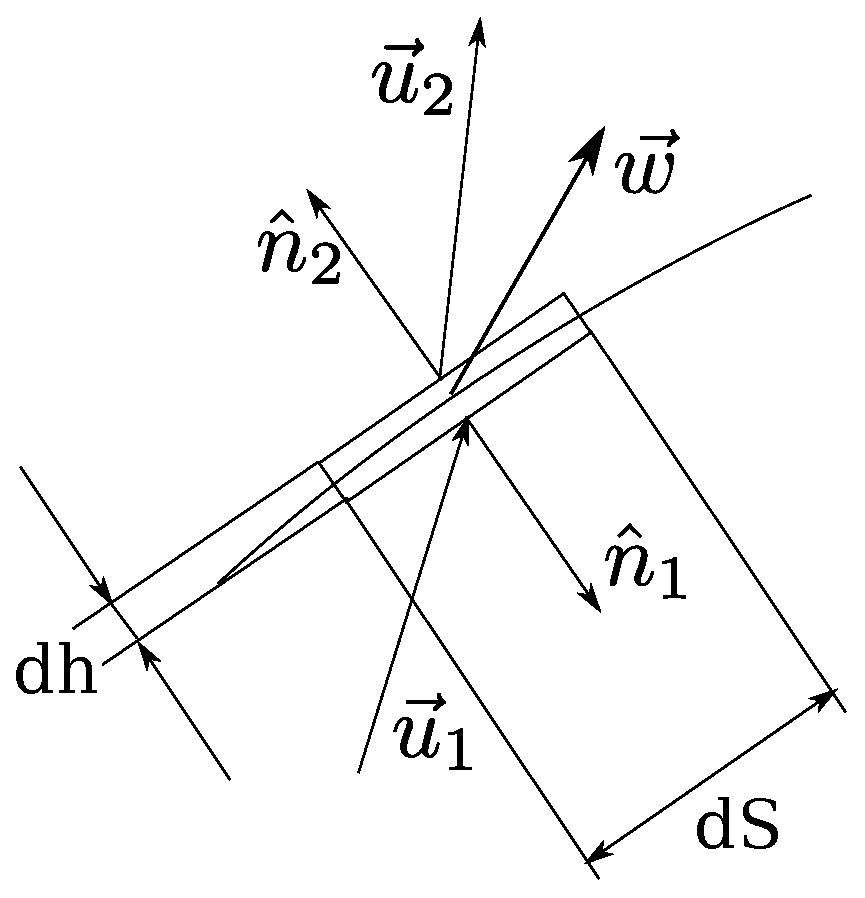
\includegraphics[width=0.30\textwidth]{./fig/elem_velocity.eps}} \qquad \qquad
\subfloat[][Definizione degli sforzi e della tensione superficiale agenti sull'elemento infinitesimo della superficie. ]
   {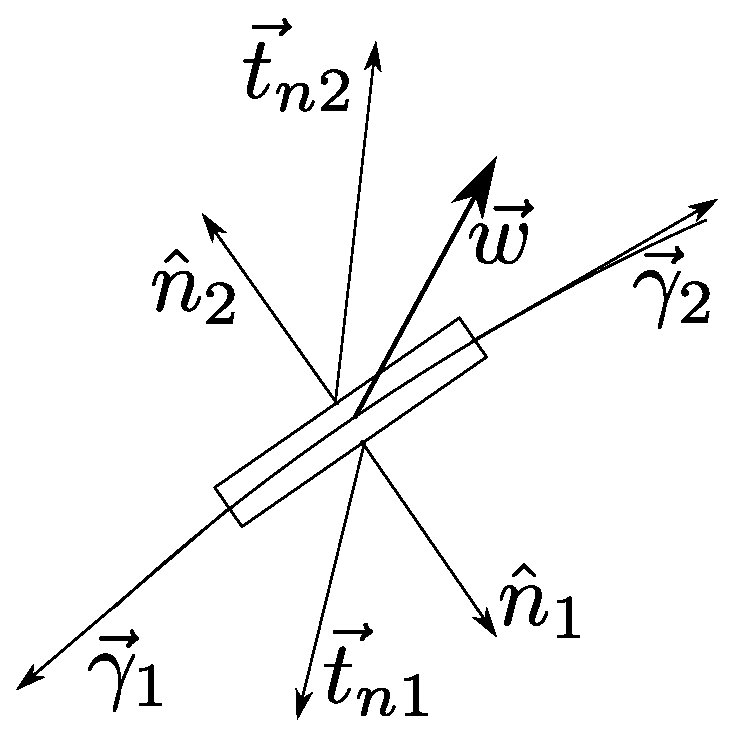
\includegraphics[width=0.30\textwidth]{./fig/elem_stress.eps}}
\end{figure}

L'elemento di volume $dv$ è il parallelepipedo di superfici laterali $dS$, paralleli alla superficie, e basi $dh$ perpendicolari
 alla superficie. Se si ipotizza che le superfici $dh \ll dS$ i contributi nei bilanci dei termini agenti sulle superfici $dh$
 (tranne che nel caso della tensione superficiale, che ha le dimensioni di uno sforzo per una lunghezza) sono trascurabili.


\subsection{Bilancio di massa}
Il bilancio di massa per il volume $dv$  in moto con velocità $\bm{w}$ è
\begin{equation}
 \dfrac{d}{dt}\int_{v} \rho + \oint_{\partial v} \rho (\bm{u} - \bm{w} ) \cdot \bm{\hat{n}} = 0
\end{equation}
Trascurando i contributi di volume e quelli delle superfici $dh$
\begin{equation}
 \rho_1 (\bm{u}_1 - \bm{w} ) \cdot \bm{\hat{n}}_1 dS +  \rho_2 (\bm{u}_2 - \bm{w} ) \cdot \bm{\hat{n}}_2 dS = 0
\end{equation}
dove le normali $\bm{\hat{n}}_1 = \bm{\hat{n}}$ e $\bm{\hat{n}}_2 = -\bm{\hat{n}}$ sono opposte. La quantità tra parentesi è la velocità relativa
 del fluido rispetto alla superficie. Si definisce quindi il flusso di massa $m$ attraverso la superficie.
\begin{equation}
\begin{aligned}
 - m & = \rho_1 (\bm{u}_1 - \bm{w} ) \cdot \bm{\hat{n}} = \rho_2 (\bm{u}_2 - \bm{w} ) \cdot \bm{\hat{n}} \\
   & = \rho_1  \bm{u}_{r1} \cdot \bm{\hat{n}} = \rho_2 \bm{u}_{r2} \cdot \bm{\hat{n}} \\
\end{aligned}
\end{equation}

\noindent
Nel caso di densità uniforme $\rho_1 = \rho_2 = \rho$ si ``conservano'' le componenti normali della velocità relativa e della
 velocità.
\begin{equation}
\begin{aligned}
  \bm{u}_{r1} \cdot \bm{\hat{n}} & = \bm{u}_{r2} \cdot \bm{\hat{n}} \\
  \bm{u}_{1}  \cdot \bm{\hat{n}} & = \bm{u}_{2}  \cdot \bm{\hat{n}} \\
\end{aligned}
\end{equation}


\subsection{Bilancio di quantità di moto}
Il bilancio della quantità di moto per l'elemento $dv$ è
\begin{equation}
 \dfrac{d}{dt}\int_{v} \rho\bm{u} + \oint_{\partial v} \rho \bm{u}(\bm{u} - \bm{w} ) \cdot \bm{\hat{n}} = \oint_{\partial v} \bm{t_n} + \int_{v} \rho \bm{g} + \int_{l} \bm{\gamma}
\end{equation}
avendo incluso anche eventuali termini di tensione superficiale, svolto 
 sulla curva che separa tre sostanze (come ad esempio il ``perimetro''
 del menisco visto nell'esercizio sul capillare: in quel caso la curva
 $l$ separa il liquido, dall'aria, dalle pareti solide del capillare).
Trascurando i termini di volume, il bilancio per l'elemento infinitesimo (per semplicità pensato in 2 dimensioni) è
\begin{equation}
 \rho_1 \bm{u}_1 (\bm{u}_1 - \bm{w})\cdot \bm{\hat{n}}_1 ds + \rho_2 \bm{u}_2 (\bm{u}_2 -\bm{w}) \cdot \bm{\hat{n}}_2 ds =
    \bm{t_{n1}} ds + \bm{\gamma}_1  + \bm{t_{n2}} ds + \bm{\gamma}_2 
\end{equation}
con $\bm{\gamma}_1 = \gamma \bm{\hat{t}_1}$, $\bm{\gamma}_2 = (\gamma + \gamma_{/s} ds) \bm{\hat{t}_2}$. I versori 
 tangenti $\bm{\hat{t}}_1$, $\bm{\hat{t}}_2$ agli estremi dell'elementino di superficie non sono allineati a causa della curvatura della superficie (si
rimanda alla ``dimostrazione'' della legge di Young-Laplace). Si tiene conto di una possibile
 variazione della tensione superficiale. Questa di solito può essere
 dovuta a differenze di temperatura o composizioni chimiche (perchè si
usa il sapone per lavarsi le mani?): si rimanda al 
 simpatico (?) video delle barchette sul fondo del documento della dimostrazione
 della legge di Young-Laplace, nel quale viene usata una ``propulsione a effetto Marangoni'' per barchette di carta. Il contributo della tensione superficiale si può scrivere come
\begin{equation}
 \bm{\gamma}_2 + \bm{\gamma}_1 = (2 \gamma H \bm{\hat{n}} + \bm{\nabla}_2 \gamma )ds
\end{equation}
dove
\begin{itemize}
 \item H è la curvatura media $H = \frac{1}{2}\left(\frac{1}{R_1} + \frac{1}{R_2}\right)$ nel caso tridimensionale, che nel caso bidimensionale
 coincide con $ \frac{1}{2 R}$ (uno dei due raggi di curvatura diventa infinito).
 \item $\bm{\hat{n}}$ è il vettore normale che punta verso i centri di
 curvatura.
 \item $\bm{\nabla}_2$ è il gradiente ristretto alla superficie, tangente ad essa.
\end{itemize}

\noindent
Ricordando la definizione di $m$ e inserendola nel bilancio
\begin{equation}
 m ( \bm{u}_1 - \bm{u}_2 ) =
    \bm{t_{n1}} + \bm{t_{n2}} + 2 \gamma H \bm{\hat{n}} + \bm{\nabla}_2 \gamma
\end{equation}

\noindent
Si analizzano ora alcuni casi particolari:
\begin{itemize}
\item Statica con tensione superficiale. La velocità è nulla ovunque, i vettori di sforzo hanno solo il contributo della pressione
 $\bm{t_n} = -p \bm{\hat{n}}$. Secondo queste ipotesi, non si possono avere contributi tangenziali nemmeno a causa della tensione 
 superficiale e quindi $\gamma$ deve essere uniforme sulla superficie. Nel caso bidimensionale si ricorda che la normale $\bm{\hat{n}}$
 punta verso il centro del cerchio osculatore e coincide quindi con la normale $\bm{\hat{n}}_1$ dell'immagine e il raggio di curvatura $R$ è positivo.
 Il bilancio della quantità di moto si riduce all'equilibrio statico della superficie
 \begin{equation}
   p_1 - p_2 = \frac{\gamma}{R}
 \end{equation}
 Si osserva quindi che la pressione ``interna'' $p_1$ deve essere maggiore di $p_2$.
\item Fluido inviscido, superficie senza tensione superficiale. Il bilancio si riduce a 
\begin{equation}
  m ( \bm{u}_1 - \bm{u}_2 ) = - (p_1 - p_2) \bm{\hat{n}}
\end{equation}
\item Fluido inviscido, superficie senza tensione superficiale, densità uniforme. Si è visto come la 
  velocità (e le velocità relative) normali alla superficie devono essere uguali da entrambe le parti
  della superficie. %Se la superficie è una superficie materiale, la velocità della superficie coincide
%  con quella del fluido e quindi la velocità relativa è nulla ed $m = 0$.
%  Risulta quindi che non ci può essere salto di pressione attraverso una tale superficie (questo è quello che significa
%  l'ipotesi espressa in termini pittoreschi di ``scia scarica'' nell'aerodinamica a potenziale).
%  \begin{equation}
%    p_1 = p_2
%  \end{equation}
  Se si ipotizza che la superifice non sia attraversata da flusso di massa (si impone che la componente normale della velocità relativa sia nulla,
  non la velocità relativa nel suo complesso). In questo caso non è possibile trovare una relazione 
  di salto per la velocità tangenziale (o almeno questo non è possibile se non si aggiungono altre ipotesi o altre equazioni \dots vedremo 
  un caso semplificato applicando il teorema di Bernoulli a un problema aerodinamico bidimensionale stazionario \dots):
  poichè $m=0$ la superficie è ``scarica'' (capiterà nei prossimi corsi di sentir parlare o aver direttamente a che fare con ``
  l'ipotesi di scia scarica'': questa non dovrà quindi essere una novità o una sorpresa in futuro)
  \begin{equation}
    p_1 = p_2
  \end{equation}
  ma non si riesce a ricavare nessuna informazione dalla componente tangenziale
  dell'equazione poichè è un'identità $0=0$ a prescindere dal valore di $( \bm{u}_1 - \bm{u}_2 )\cdot \bm{\hat{t}}$. Attraverso tale superficie
  (di spessore nullo) ci può essere un salto finito di velocità tangenziale: in questo caso la superficie è una superficie di vorticità infinita
\end{itemize}

\noindent
L'ultimo caso particolare verrà utilizzato in qualche esercizio in cui un dominio occupato da un fluido può essere suddiviso in un sottodominio 
 nel quale è valido il teorema di Bernoulli (in qualche forma \dots) e in un sottodominio dove sono valide le relazioni della statica: le condizioni
 di salto serviranno a far comunicare tra di loro i due sottodomini (e a risolvere correttamente l'esercizio).

\subsection{Bilancio di energia}
Non verrà detto nulla sulle relazioni di salto delle altre quantità \dots



